% En el preámbulo:
% \usepackage{tikz}
% \usetikzlibrary{arrows.meta,calc}

\newcommand{\coordSaneamiento}{
\coordinate (A) at (0,4);
\coordinate (B) at (2,5);
\coordinate (C) at (3,3.8);
\coordinate (D) at (1,2.4);
\coordinate (E) at (4.2,5.1);
\coordinate (F) at (5.0,3.7);
\coordinate (G) at (4.0,2.2);
\coordinate (H) at (6.5,5.0);
\coordinate (I) at (7.2,3.6);
\coordinate (J) at (6.2,2.1);
}

\newcommand{\aristasSaneamiento}{
\draw[arista] (A)--(B);
\draw[arista] (A)--(C);
\draw[arista] (A)--(D);
\draw[arista] (B)--(C);
\draw[arista] (B)--(E);
\draw[arista] (C)--(D);
\draw[arista] (C)--(F);
\draw[arista] (D)--(G);
\draw[arista] (E)--(F);
\draw[arista] (E)--(H);
\draw[arista] (F)--(G);
\draw[arista] (F)--(I);
\draw[arista] (G)--(J);
\draw[arista] (H)--(I);
\draw[arista] (I)--(J);
}

\newcommand{\pesosSaneamiento}{
\path (A)--node[peso]{$90$}(B);
\path (A)--node[peso]{$120$}(C);
\path (A)--node[peso]{$110$}(D);
\path (B)--node[peso]{$80$}(C);
\path (B)--node[peso]{$100$}(E);
\path (C)--node[peso]{$70$}(D);
\path (C)--node[peso]{$95$}(F);
\path (D)--node[peso]{$85$}(G);
\path (E)--node[peso]{$75$}(F);
\path (E)--node[peso]{$60$}(H);
\path (F)--node[peso]{$60$}(G);
\path (F)--node[peso]{$50$}(I);
\path (G)--node[peso]{$80$}(J);
\path (H)--node[peso]{$70$}(I);
\path (I)--node[peso]{$65$}(J);
}

\newcommand{\nodosSaneamiento}{
\foreach \n in {A,B,C,D,E,F,G,H,I,J}{
\node[vertice] at (\n) {$\n$};
}
}

\newcommand{\nodosImparesSaneamiento}{
\foreach \n in {A,B,D,E,G,I}{
\node[verticeSol] at (\n) {$\mathbf{\n}$};
}
}

\newcommand{\nodosTodosSaneamiento}{
\foreach \n in {A,B,C,D,E,F,G,H,I,J}{
\node[verticeSol] at (\n) {$\mathbf{\n}$};
}
}

\tikzset{
vertice/.style={circle,draw,fill=white,minimum size=5mm,inner sep=0pt,font=\scriptsize},
verticeSol/.style={circle,draw,very thick,fill=white,minimum size=5mm,inner sep=0pt,font=\scriptsize},
arista/.style={gray!65,line width=0.4pt},
solucion/.style={black,line width=1.8pt},
duplicada/.style={black,line width=1.5pt,dashed},
peso/.style={font=\tiny,fill=white,inner sep=1pt,sloped,above}
}

\textbf{Solución}

El problema planteado es un problema del cartero chino no dirigido. Se debe recorrer cada arista al menos una vez, empezando y terminando en el mismo vértice, y minimizando la distancia total recorrida. Si todos los vértices tuvieran grado par, bastaría con encontrar un circuito euleriano. Como no ocurre así, será necesario duplicar algunos caminos de longitud mínima para que todos los grados pasen a ser pares.

\begin{enumerate}
\item \textbf{Paso 1. Identificación de los vértices de grado impar.}

Se calcula el grado de cada vértice del grafo:

\[
\begin{array}{c|cccccccccc}
v & A & B & C & D & E & F & G & H & I & J\\
\hline
grado(v) & 3 & 3 & 4 & 3 & 3 & 4 & 3 & 2 & 3 & 2
\end{array}
\]

Los vértices de grado impar son:

\[
A,\ B,\ D,\ E,\ G,\ I.
\]

En el siguiente grafo se muestran en negrita los vértices de grado impar.

\begin{center}
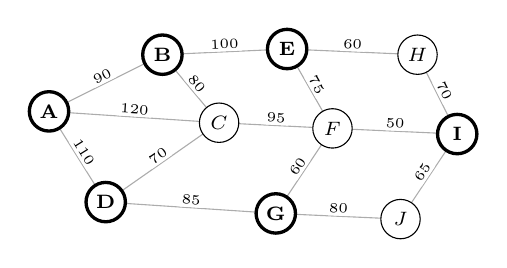
\begin{tikzpicture}[scale=0.72]
    \coordSaneamiento
    \aristasSaneamiento
    \pesosSaneamiento
    \nodosSaneamiento
    \nodosImparesSaneamiento
\end{tikzpicture}
\end{center}

Como hay vértices de grado impar, no existe un circuito euleriano que recorra cada arista exactamente una vez. Por tanto, habrá que duplicar algunos caminos para conseguir que todos los vértices tengan grado par.

\item \textbf{Paso 2. Cálculo de los caminos mínimos entre vértices impares.}

Se calculan las distancias mínimas entre todos los pares de vértices impares. La tabla de distancias mínimas es:

\[
\begin{array}{c|cccccc}
 & A & B & D & E & G & I\\
\hline
A & - & 90 & 110 & 190 & 195 & 265\\
B &   & -  & 150 & 100 & 235 & 225\\
D &   &    & -   & 220 & 85  & 195\\
E &   &    &     & -   & 135 & 125\\
G &   &    &     &     & -   & 110\\
I &   &    &     &     &     & -
\end{array}
\]

En el grafo se mantienen en negrita los vértices que deben emparejarse mediante caminos mínimos.

\begin{center}
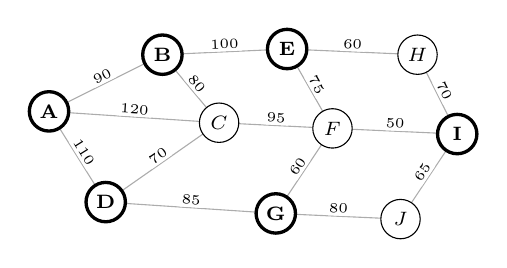
\begin{tikzpicture}[scale=0.72]
    \coordSaneamiento
    \aristasSaneamiento
    \pesosSaneamiento
    \nodosSaneamiento
    \nodosImparesSaneamiento
\end{tikzpicture}
\end{center}

\item \textbf{Paso 3. Emparejamiento óptimo de los vértices impares.}

Hay que emparejar los vértices impares de dos en dos, escogiendo la combinación de menor coste total. Al comparar las posibles combinaciones, se obtiene:

\[
\begin{array}{c|c}
\text{Emparejamiento} & \text{Coste}\\
\hline
(A,B), (D,G), (E,I) & 90+85+125=300\\
(A,D), (B,E), (G,I) & 110+100+110=320\\
(A,B), (D,E), (G,I) & 90+220+110=420\\
(A,B), (D,I), (E,G) & 90+195+135=420\\
(A,E), (B,D), (G,I) & 190+150+110=450\\
(A,I), (B,E), (D,G) & 265+100+85=450
\end{array}
\]

La combinación de menor coste es:

\[
(A,B),\quad (D,G),\quad (E,I),
\]

con coste total adicional:

\[
90+85+125=300.
\]

El camino mínimo entre $E$ e $I$ es:

\[
E-F-I,
\]

con longitud:

\[
75+50=125.
\]

Por tanto, los tramos que deben duplicarse son:

\[
AB,\quad DG,\quad EF,\quad FI.
\]

En el grafo se muestran en negrita los caminos que se incorporan a la solución.

\begin{center}
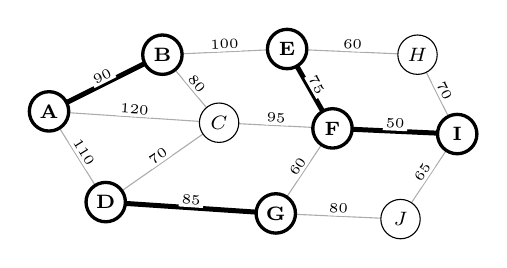
\begin{tikzpicture}[scale=0.72]
    \coordSaneamiento
    \aristasSaneamiento

    \draw[solucion] (A)--(B);
    \draw[solucion] (D)--(G);
    \draw[solucion] (E)--(F);
    \draw[solucion] (F)--(I);

    \pesosSaneamiento
    \nodosSaneamiento
    \nodosImparesSaneamiento
    \node[verticeSol] at (F) {$\mathbf{F}$};
\end{tikzpicture}
\end{center}

\item \textbf{Paso 4. Construcción del grafo euleriano.}

Se duplican los tramos $AB$, $DG$, $EF$ y $FI$. Con ello, todos los vértices pasan a tener grado par y el grafo resultante admite un circuito euleriano.

La longitud total original de la red es:

\[
\begin{aligned}
L
&=90+120+110+80+100+70+95+85\\
&\quad +75+60+60+50+80+70+65\\
&=1210.
\end{aligned}
\]

La longitud adicional mínima que hay que recorrer es:

\[
300.
\]

Por tanto, la distancia total mínima será:

\[
1210+300=1510.
\]

En el siguiente grafo se representan con trazo discontinuo y en negrita los tramos duplicados.

\begin{center}
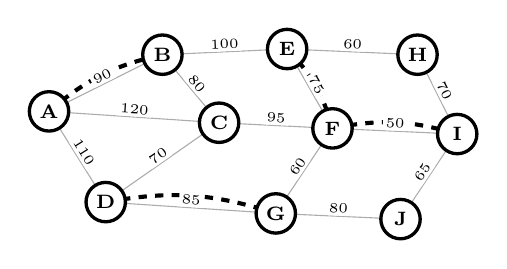
\begin{tikzpicture}[scale=0.72]
    \coordSaneamiento
    \aristasSaneamiento

    \draw[duplicada] (A) to[bend left=14] (B);
    \draw[duplicada] (D) to[bend left=14] (G);
    \draw[duplicada] (E) to[bend left=14] (F);
    \draw[duplicada] (F) to[bend left=14] (I);

    \pesosSaneamiento
    \nodosSaneamiento
    \nodosTodosSaneamiento
\end{tikzpicture}
\end{center}

\item \textbf{Paso 5. Obtención de un recorrido óptimo.}

Una vez duplicados los tramos anteriores, se puede construir un circuito euleriano. Un recorrido óptimo posible es:

\[
A-B-E-F-I-J-G-D-G-F-I-H-E-F-C-D-A-C-B-A.
\]

Este recorrido empieza y termina en $A$ y recorre todos los tramos de la red al menos una vez. Además, solo repite los tramos necesarios para hacer que el grafo sea euleriano.

La distancia total recorrida es:

\[
\begin{aligned}
&90+100+75+50+65+80+85+85+60+50\\
&\quad +70+60+75+95+70+110+120+80+90\\
&=1510.
\end{aligned}
\]

En el grafo se muestran de nuevo en negrita los tramos duplicados que hacen posible el circuito euleriano.

\begin{center}
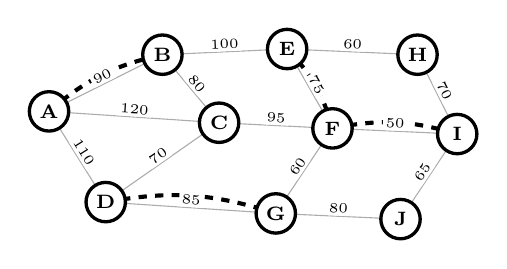
\begin{tikzpicture}[scale=0.72]
    \coordSaneamiento
    \aristasSaneamiento

    \draw[duplicada] (A) to[bend left=14] (B);
    \draw[duplicada] (D) to[bend left=14] (G);
    \draw[duplicada] (E) to[bend left=14] (F);
    \draw[duplicada] (F) to[bend left=14] (I);

    \pesosSaneamiento
    \nodosSaneamiento
    \nodosTodosSaneamiento
\end{tikzpicture}
\end{center}

Por tanto, la distancia total mínima que debe recorrer el equipo de inspección es:

\[
\boxed{1510\text{ metros}}.
\]

Un recorrido óptimo es:

\[
\boxed{A-B-E-F-I-J-G-D-G-F-I-H-E-F-C-D-A-C-B-A}.
\]


\end{enumerate}
